\documentclass[12pt,pdf,hyperref={unicode}]{beamer}


%\documentclass[10pt]{beamer}

\usetheme[progressbar=frametitle]{metropolis}

\usepackage{booktabs}
\usepackage[scale=2]{ccicons}

\usepackage{pgfplots}
\usepgfplotslibrary{dateplot}

\usepackage{xspace}
\newcommand{\themename}{\textbf{\textsc{metropolis}}\xspace}


%\usepackage{lmodern}

% подключаем кириллицу 
\usepackage[T2A]{fontenc}
\usepackage[utf8]{inputenc}
\usepackage{listings}
%\usepackage{graphicx}
\usepackage{hyperref}

% отключить клавиши навигации
\setbeamertemplate{navigation symbols}{}

% тема оформления
\usetheme{Pittsburgh}

% цветовая схема
\usecolortheme{default}

\definecolor{light-gray}{gray}{0.90}

\title{Семинар №3}   
\subtitle{ФАКИ \the\year}
\author{Бирюков В. А.} 
\date{\today} 
% \logo{
\includegraphics[height=5mm]{images/logo.png}\vspace{-7pt}}

\begin{document}

\lstset{language=C}

% титульный слайд
\begin{frame}
\titlepage
\end{frame} 

\defverbatim[colored]\makeset{
\begin{lstlisting}[language=C++,basicstyle=\ttfamily,keywordstyle=\color{blue}]
void make_set(int X) {
  parent[X] = X;
}
\end{lstlisting}
}

\lstset{
  language=C,                % choose the language of the code
  basicstyle=\ttfamily,
  columns=fixed,
  fontadjust=true,
  basewidth=0.5em,
  keywordstyle=\color{blue}\bfseries,
  commentstyle=\color{gray},
  stringstyle=\ttfamily\color{yellow!40!red},
  showstringspaces=false,
  %numbers=false,                   % where to put the line-numbers
  numbersep=5pt,
  numberstyle=\tiny\color{gray},
  numberfirstline=true,
  stepnumber=1,                   % the step between two line-numbers.        
  numbersep=5pt,                  % how far the line-numbers are from the code
  backgroundcolor=\color{white!90!gray},  % choose the background color. You must add \usepackage{color}
  showstringspaces=false,         % underline spaces within strings
  captionpos=b,                   % sets the caption-position to bottom
  breaklines=true,                % sets automatic line breaking
  breakatwhitespace=true,         % sets if automatic breaks should only happen at whitespace
}
\lstset{literate=%
   *{0}{{{\color{red!20!violet}0}}}1
    {1}{{{\color{red!20!violet}1}}}1
    {2}{{{\color{red!20!violet}2}}}1
    {3}{{{\color{red!20!violet}3}}}1
    {4}{{{\color{red!20!violet}4}}}1
    {5}{{{\color{red!20!violet}5}}}1
    {6}{{{\color{red!20!violet}6}}}1
    {7}{{{\color{red!20!violet}7}}}1
    {8}{{{\color{red!20!violet}8}}}1
    {9}{{{\color{red!20!violet}9}}}1
}


\section{Объявление, определение и вызов функций}

\begin{frame}[fragile]
\frametitle{Функции} 

\begin{itemize}
\item Функция -- фрагмент программного кода, к которому можно обратиться из другого места программы
\item Функция должна быть соответствующим образом \textbf{объявлена} и \textbf{определена}
\end{itemize}

\end{frame}

\begin{frame}[fragile]
\frametitle{Объявление функций(прототипы функций)} 
\begin{itemize}
\item Как и переменная, функция также должна объявлена перед использованием
\item Определение функции называется прототипом функции
\item Пример прототипа:\\
\begin{lstlisting}
int sum (int a, int b)
\end{lstlisting}
или:
\begin{lstlisting}
int sum (int , int)
\end{lstlisting}
\end{itemize}
\end{frame}


\begin{frame}[fragile]
\frametitle{Вызов функций} 
\begin{itemize}
\item Примеры вызова функции:\\
Функция, определяемая пользователем:\\
\begin{lstlisting}
sum(a, b)
\end{lstlisting}
Библиотечные функции:\\
\begin{lstlisting}
sqrt(x)
\end{lstlisting}
\begin{lstlisting}
printf("%d\n", a)
\end{lstlisting}
\end{itemize}
\end{frame}



\begin{frame}[fragile]
\frametitle{Определение функции} 
\begin{center}
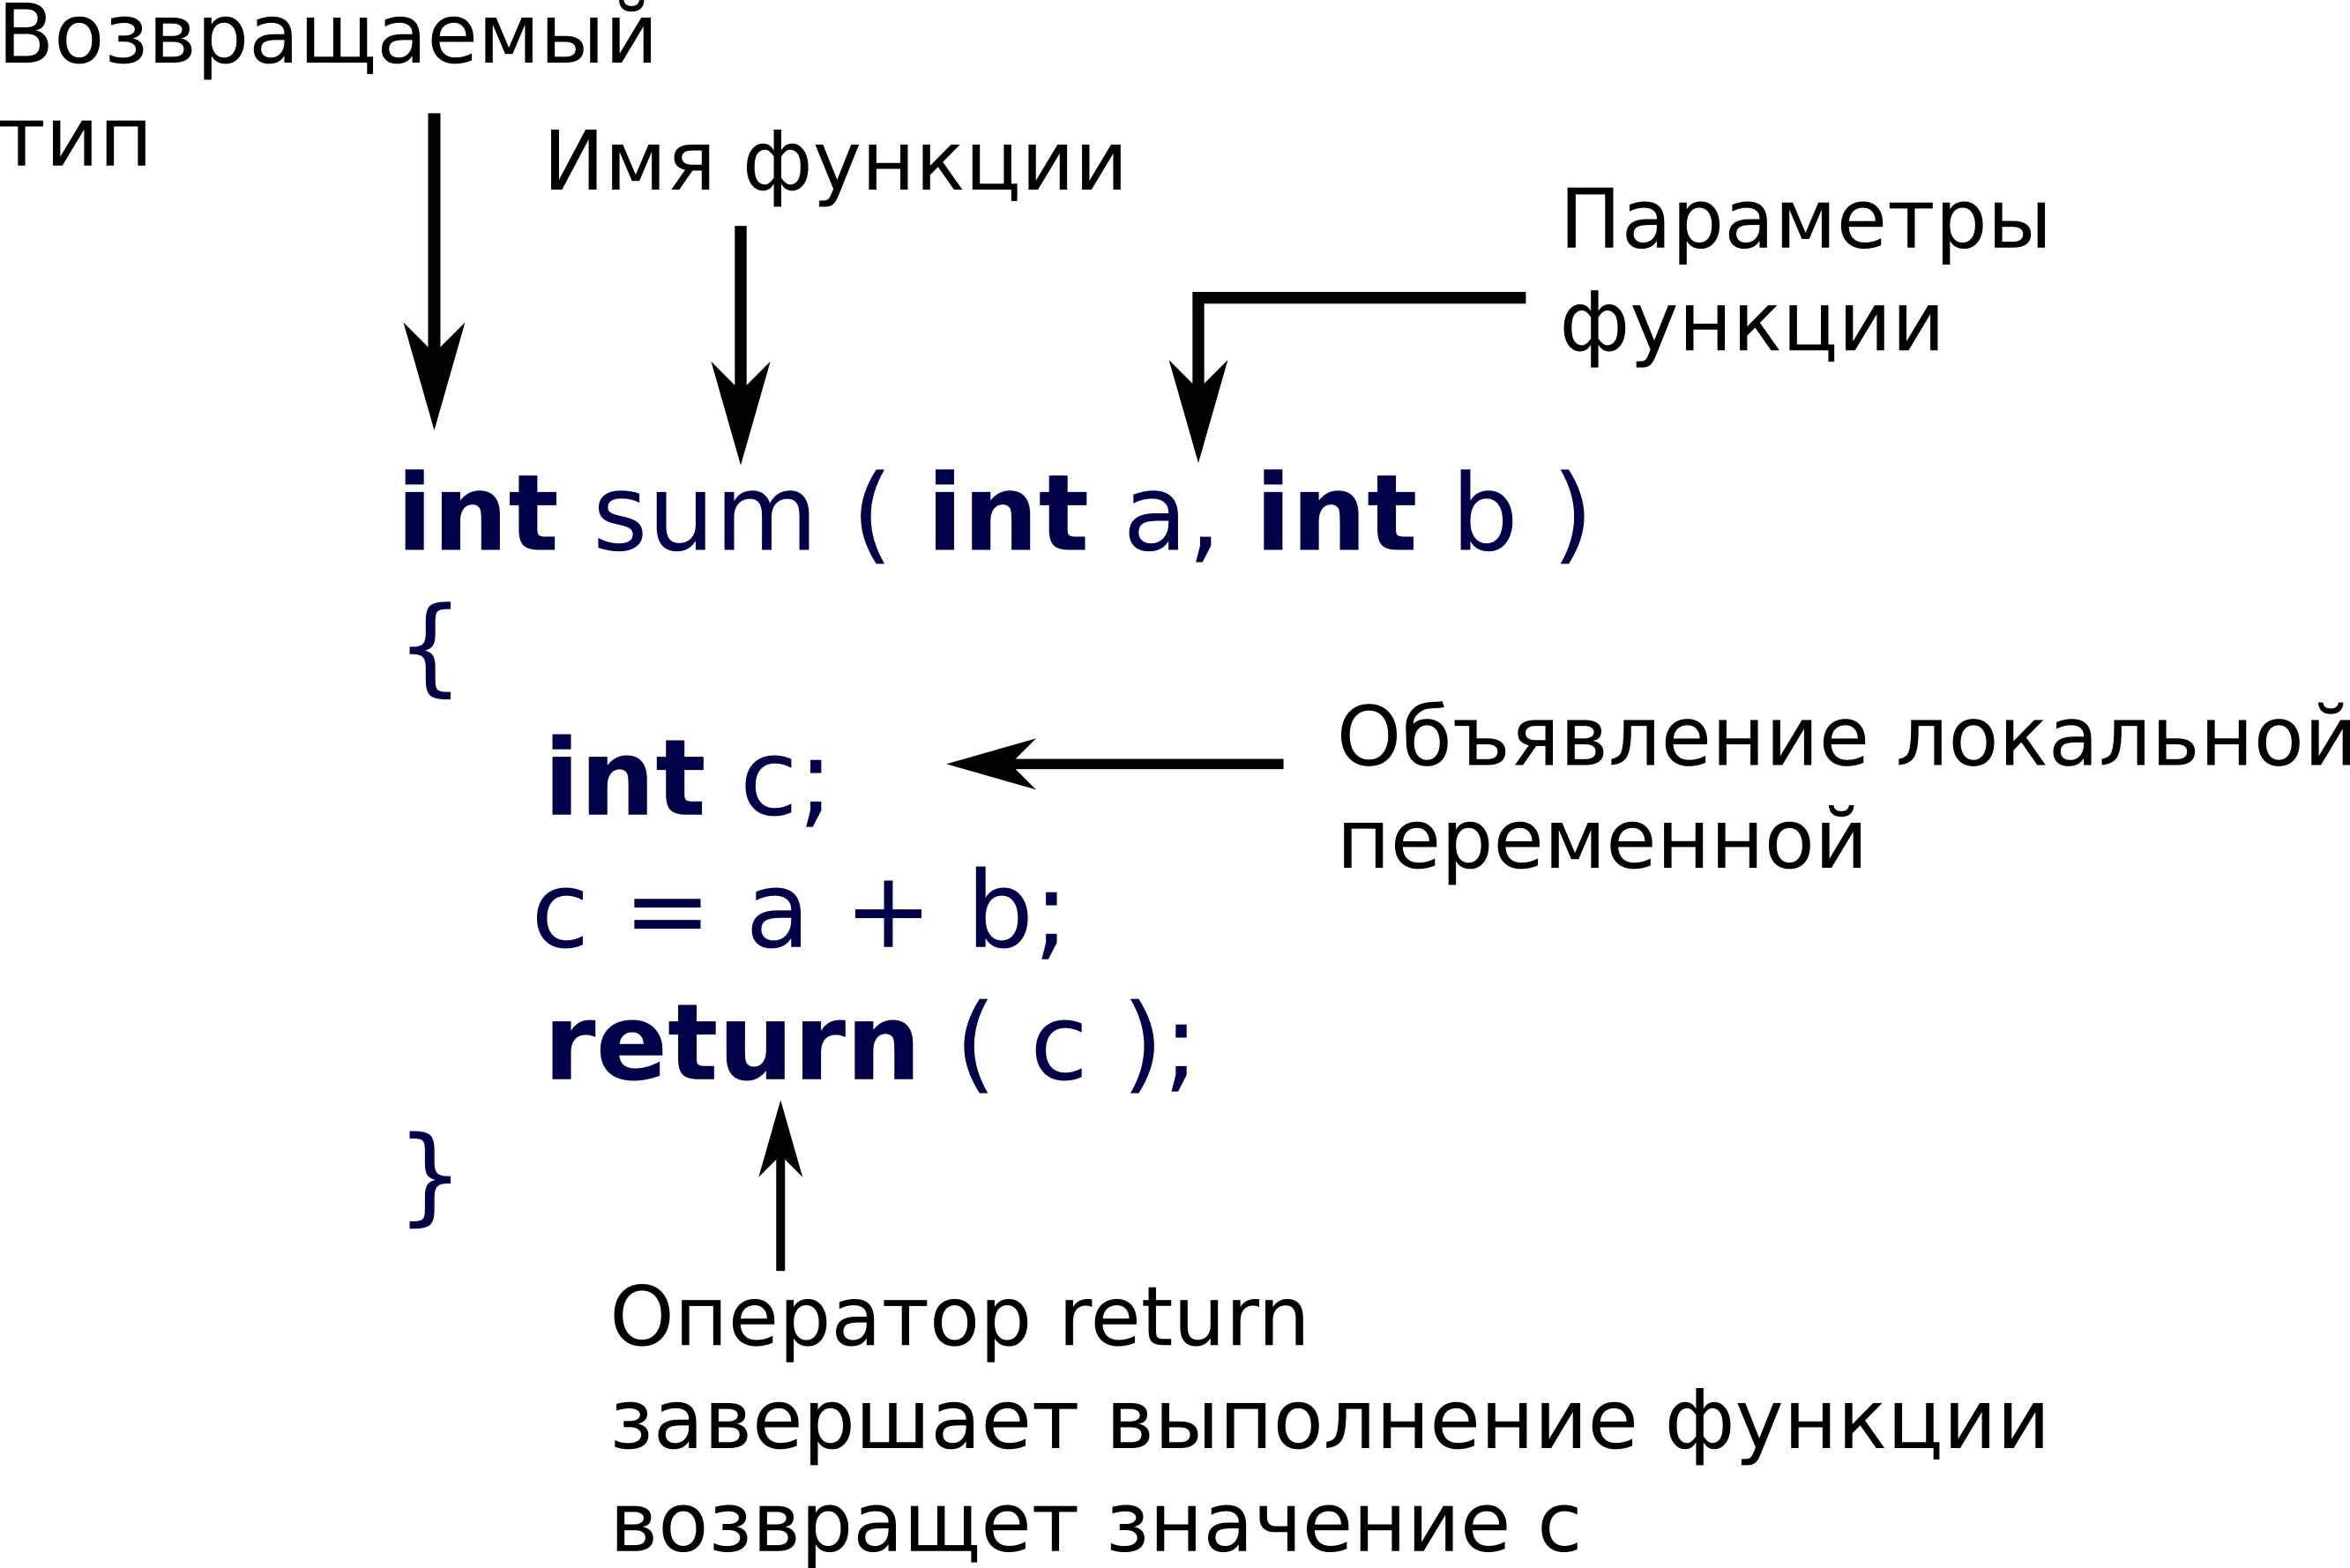
\includegraphics[width=0.8\linewidth]{images/function_syntax.png}
\end{center}
\end{frame}

\begin{frame}[fragile]
\frametitle{Функции} 
\begin{center}
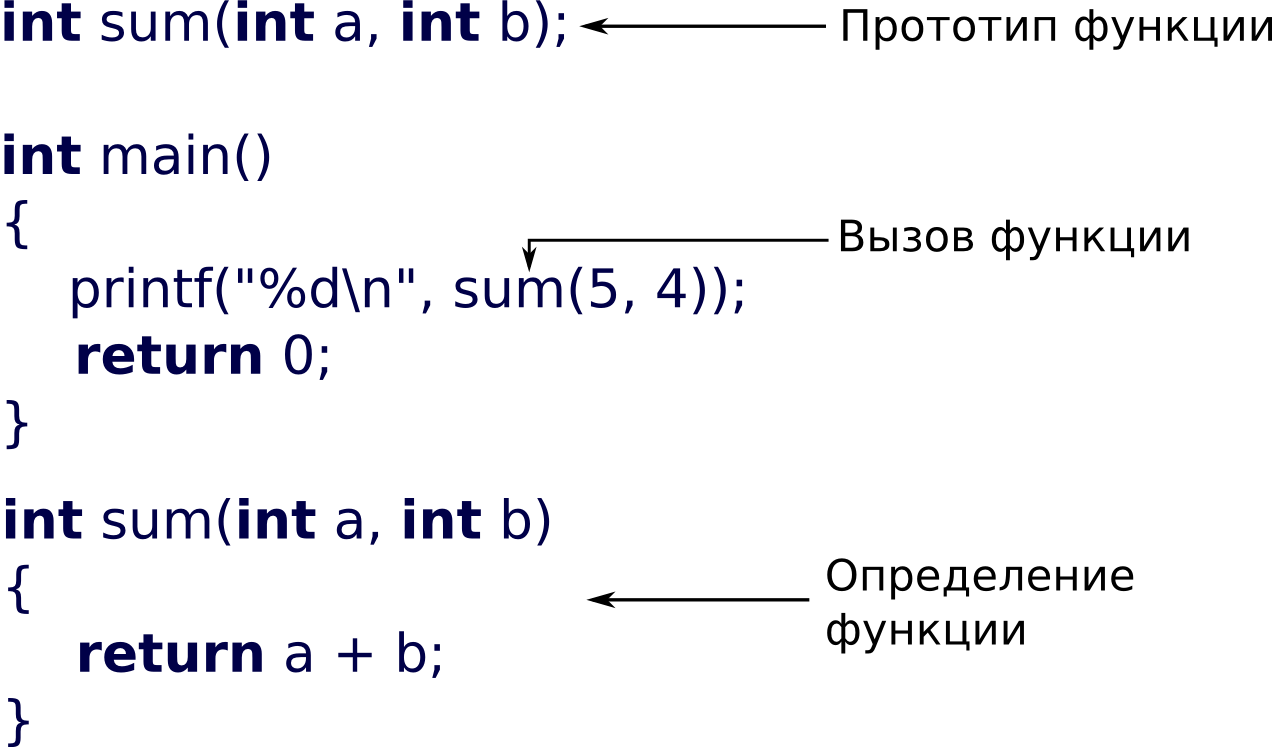
\includegraphics[width=0.8\linewidth]{images/function_summary.png}
\end{center}
\end{frame}

\begin{frame}[fragile]
\frametitle{Функции} 
\begin{center}
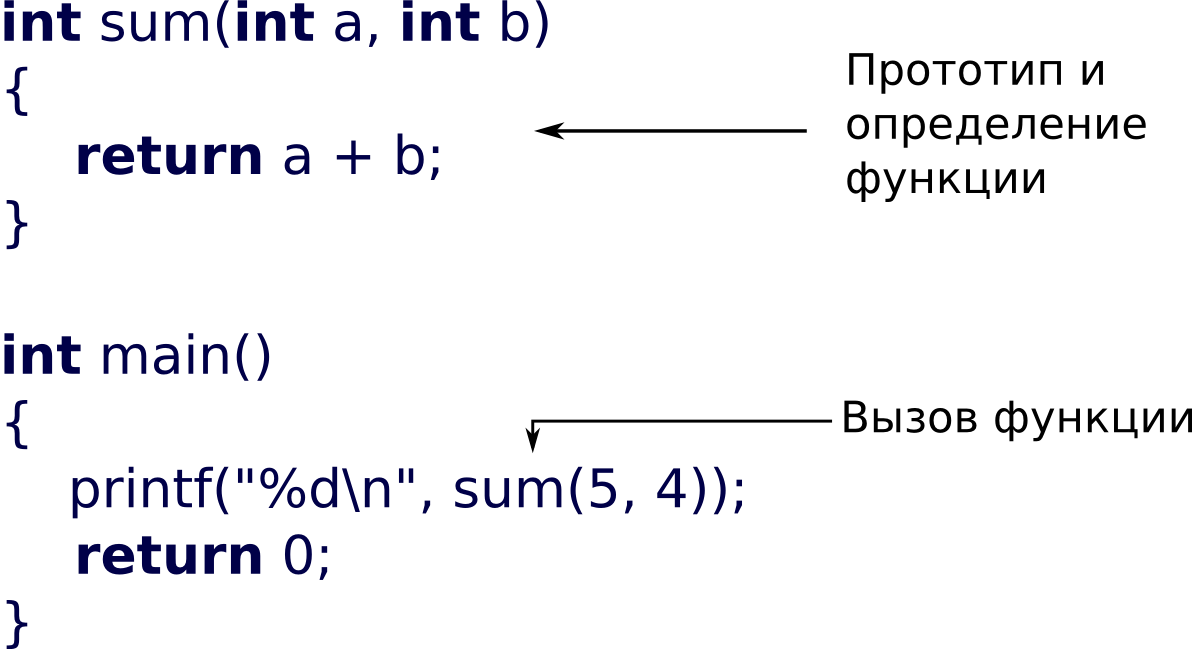
\includegraphics[width=0.8\linewidth]{images/function_summary2.png}

Зачем разделять прототип функции и её определение?
\end{center}
\end{frame}


\begin{frame}[fragile]
\frametitle{Спецификатор типа void} 
\begin{center}
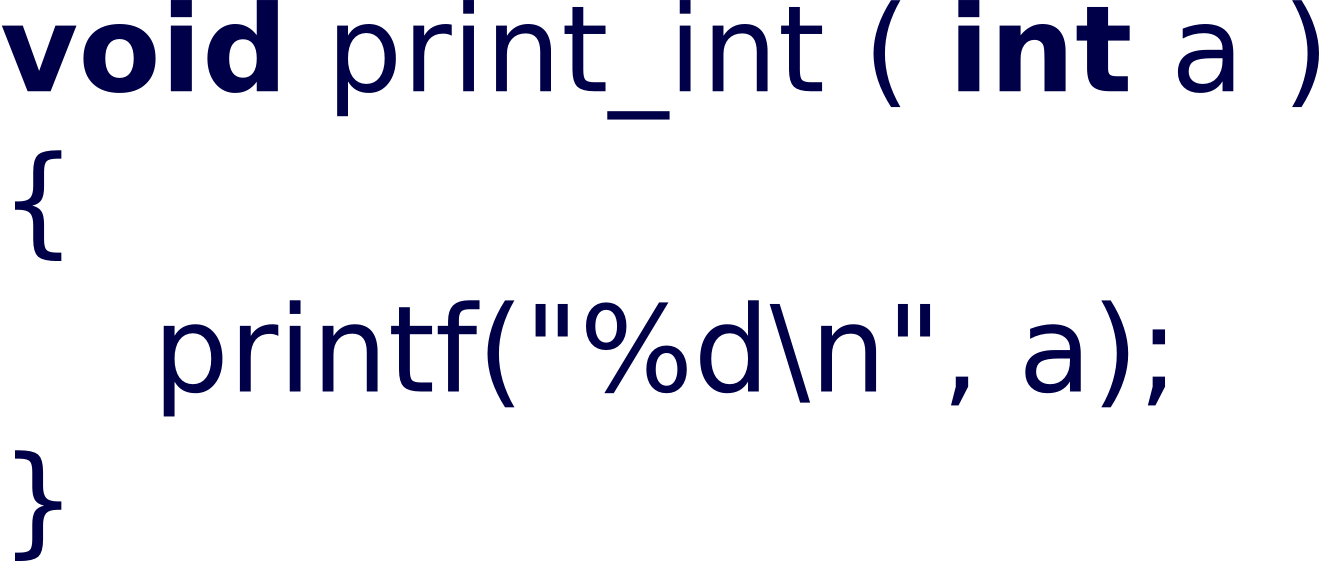
\includegraphics[width=0.45\linewidth]{images/function_void.png}
\end{center}
\begin{itemize}
\item Указывает на то, что функция ничего не возвращает
\end{itemize}
\end{frame}

\begin{frame}[fragile]
\frametitle{Спецификатор типа void} 
\begin{center}
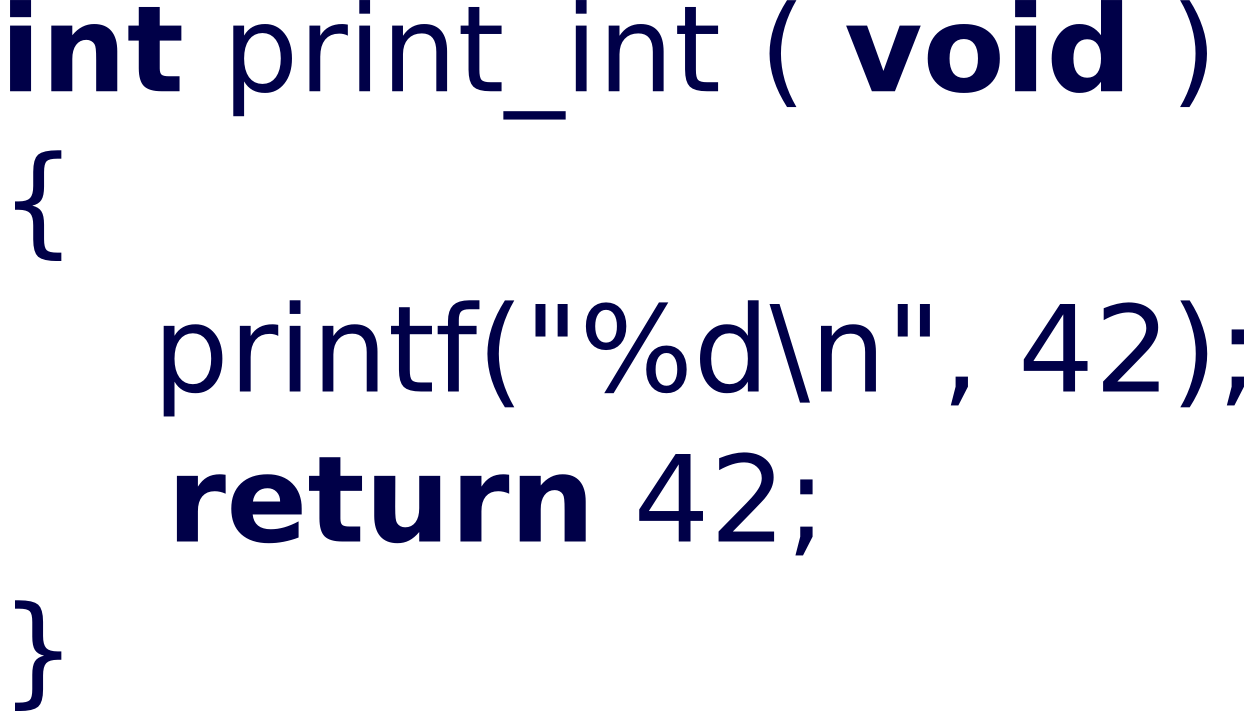
\includegraphics[width=0.45\linewidth]{images/function_void2.png}
\end{center}
\begin{itemize}
\item Указывает на то, что функция ничего не принимает
\end{itemize}
\end{frame}


\section{Области видимости переменных}

\begin{frame}[fragile]
\frametitle{Области видимости переменных} 
\begin{itemize}
\item Область видимости -- область программы, в пределах которой имя некоторой переменной продолжает быть связанным с этой переменной и возвращать её значение.
\item Глобальная переменная -- объявляются вне всех функций и доступны отовсюду
\item Локальная переменная --  объявляются внутри блока и недоступны вне его
\end{itemize}
\end{frame}

\begin{frame}[fragile]
\frametitle{Области видимости переменных} 
Функция определяет собственную (локальную) область видимости, куда входят:
\begin{enumerate}
\item Глобальные переменные
\item Входные параметры
\item Переменные, которые объявляются в теле самой функции
\end{enumerate}
\end{frame}



\section{Передача по ссылке и значению}

\begin{frame}[fragile]
\frametitle{Передача по значению} 
\begin{itemize}
\item В памяти создаётся копия передаваемого значения, которое и используется в функции
\item Значение передаваемой переменной не изменяется
\item Этот способ передачи используется в языке C
\end{itemize}
\end{frame}

\begin{frame}[fragile]
\frametitle{Передача по значению} 
\framesubtitle{Что выведет программа?} 
\begin{center}
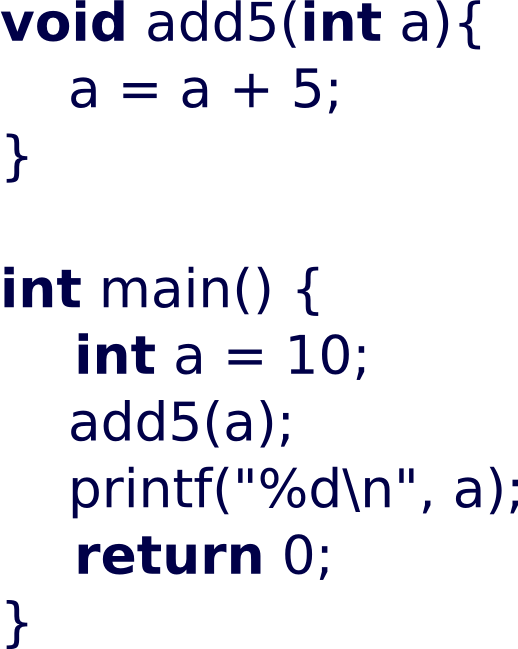
\includegraphics[width=0.4\linewidth]{images/function_passvalue.png}
\end{center}
\end{frame}

\begin{frame}[fragile]
\frametitle{Передача по ссылке} 
\begin{itemize}
\item Используется переменная, передаваемая в функцию
\item Если её значение в функции изменяется, то и изменяется значение исходной переменной
\item Этого способа передачи нет в C
\item Но можно эффективно делать почти то же самое при помощи указателей
\end{itemize}
\end{frame}

\begin{frame}[fragile]
\frametitle{Передача адресса переменной}
\framesubtitle{Что выведет программа?} 
\begin{center}
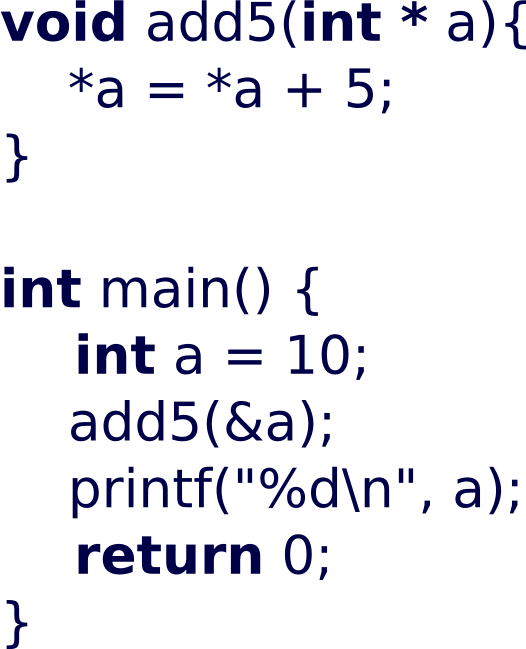
\includegraphics[width=0.4\linewidth]{images/function_passpointer.png}
\end{center}
\end{frame}


\iffalse
\section{Функция main}


\begin{frame}[fragile]
\frametitle{Функция main} 
\begin{center}
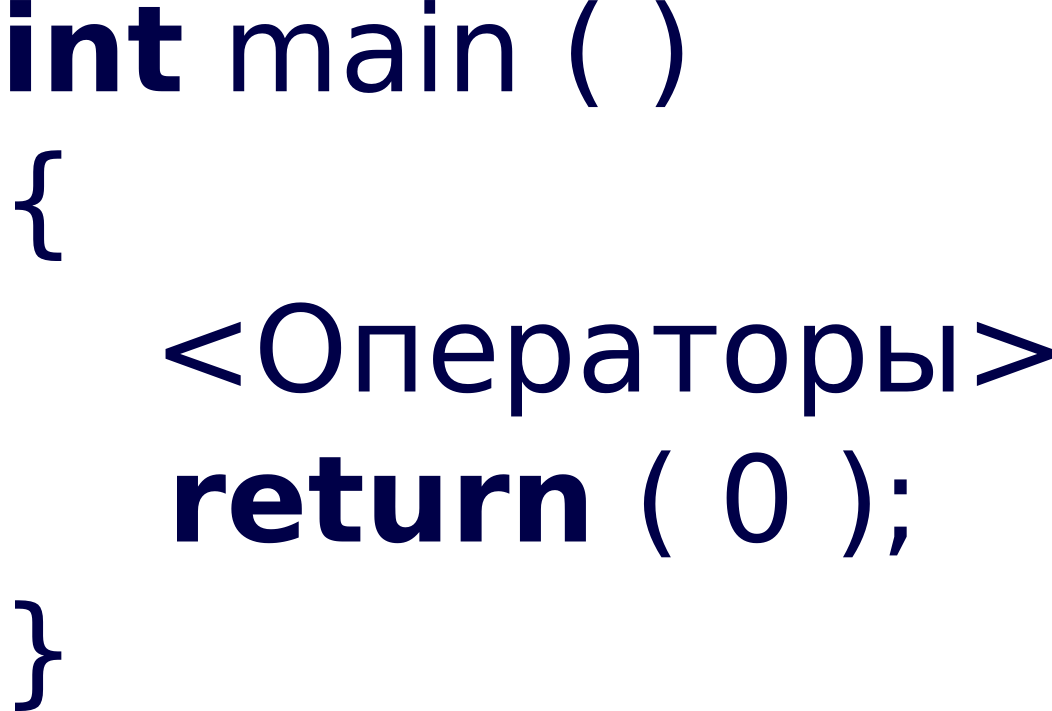
\includegraphics[width=0.35\linewidth]{images/function_syntax_main.png}
\end{center}
\begin{itemize}
\item Точка входа в программу
\item Возвращает 0, если программа завершилась нормально
\item В простейшем виде не принимает аргументов
\end{itemize}
\end{frame}


\begin{frame}[fragile]
\frametitle{Функция main}  
\begin{center}
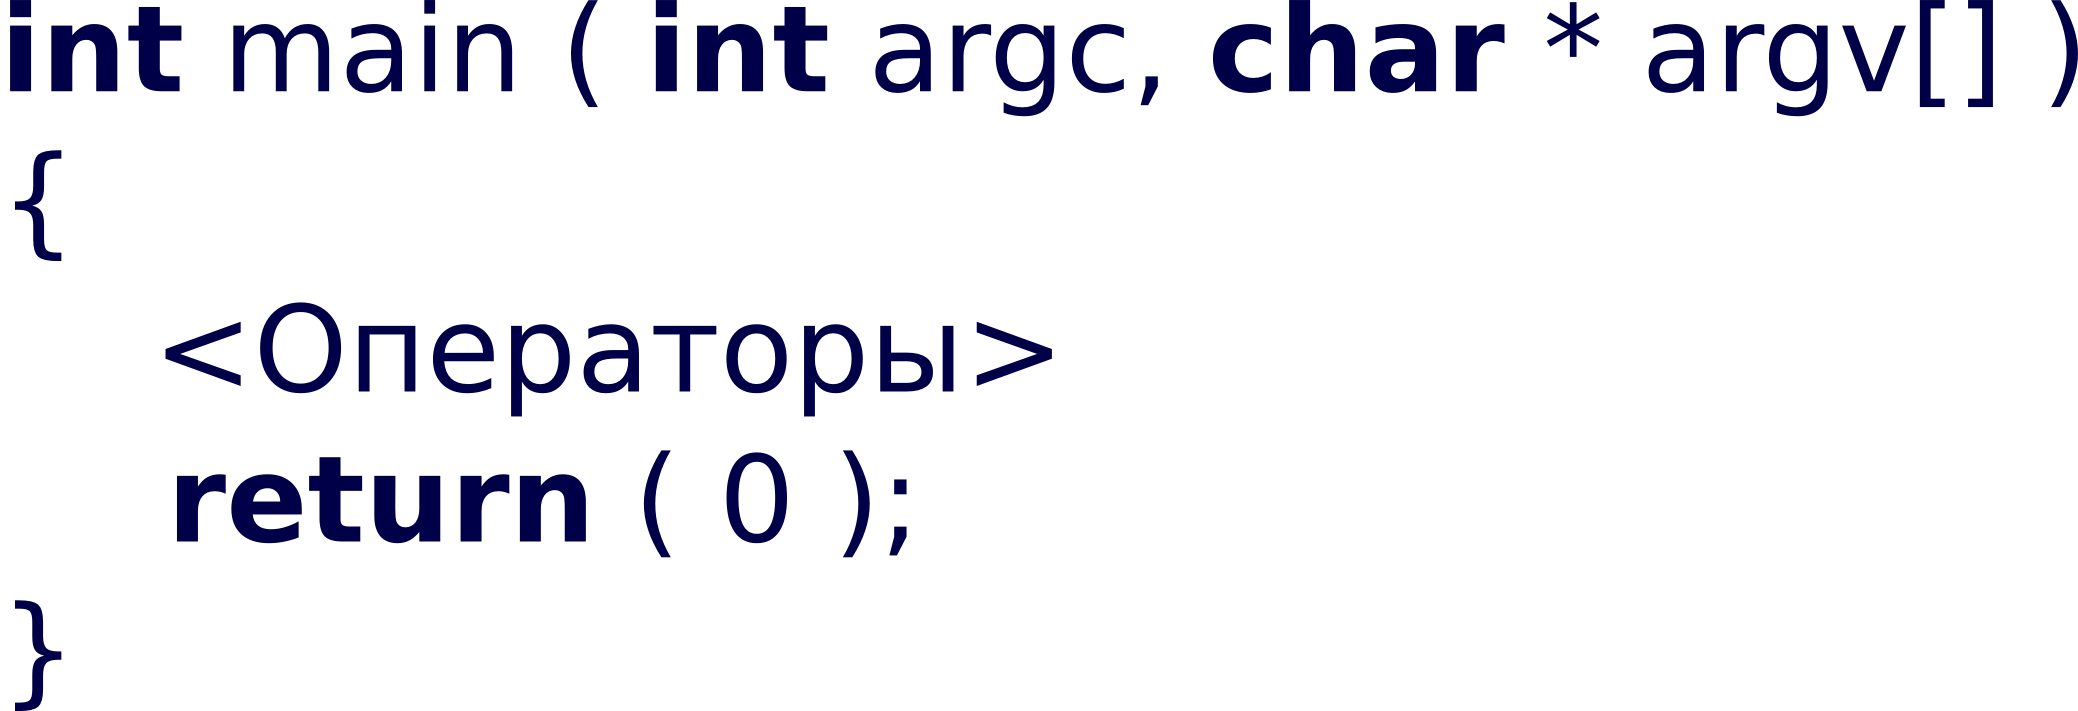
\includegraphics[width=0.7\linewidth]{images/function_syntax_main_args.png}
\end{center}
\begin{itemize}
\item argv -- параметры, передаваемые в функцию main
\item argc -- количество этих параметров
\end{itemize}
\end{frame}

\begin{frame}[fragile]
\frametitle{Функции} 
\framesubtitle{Функция main}
\begin{center}
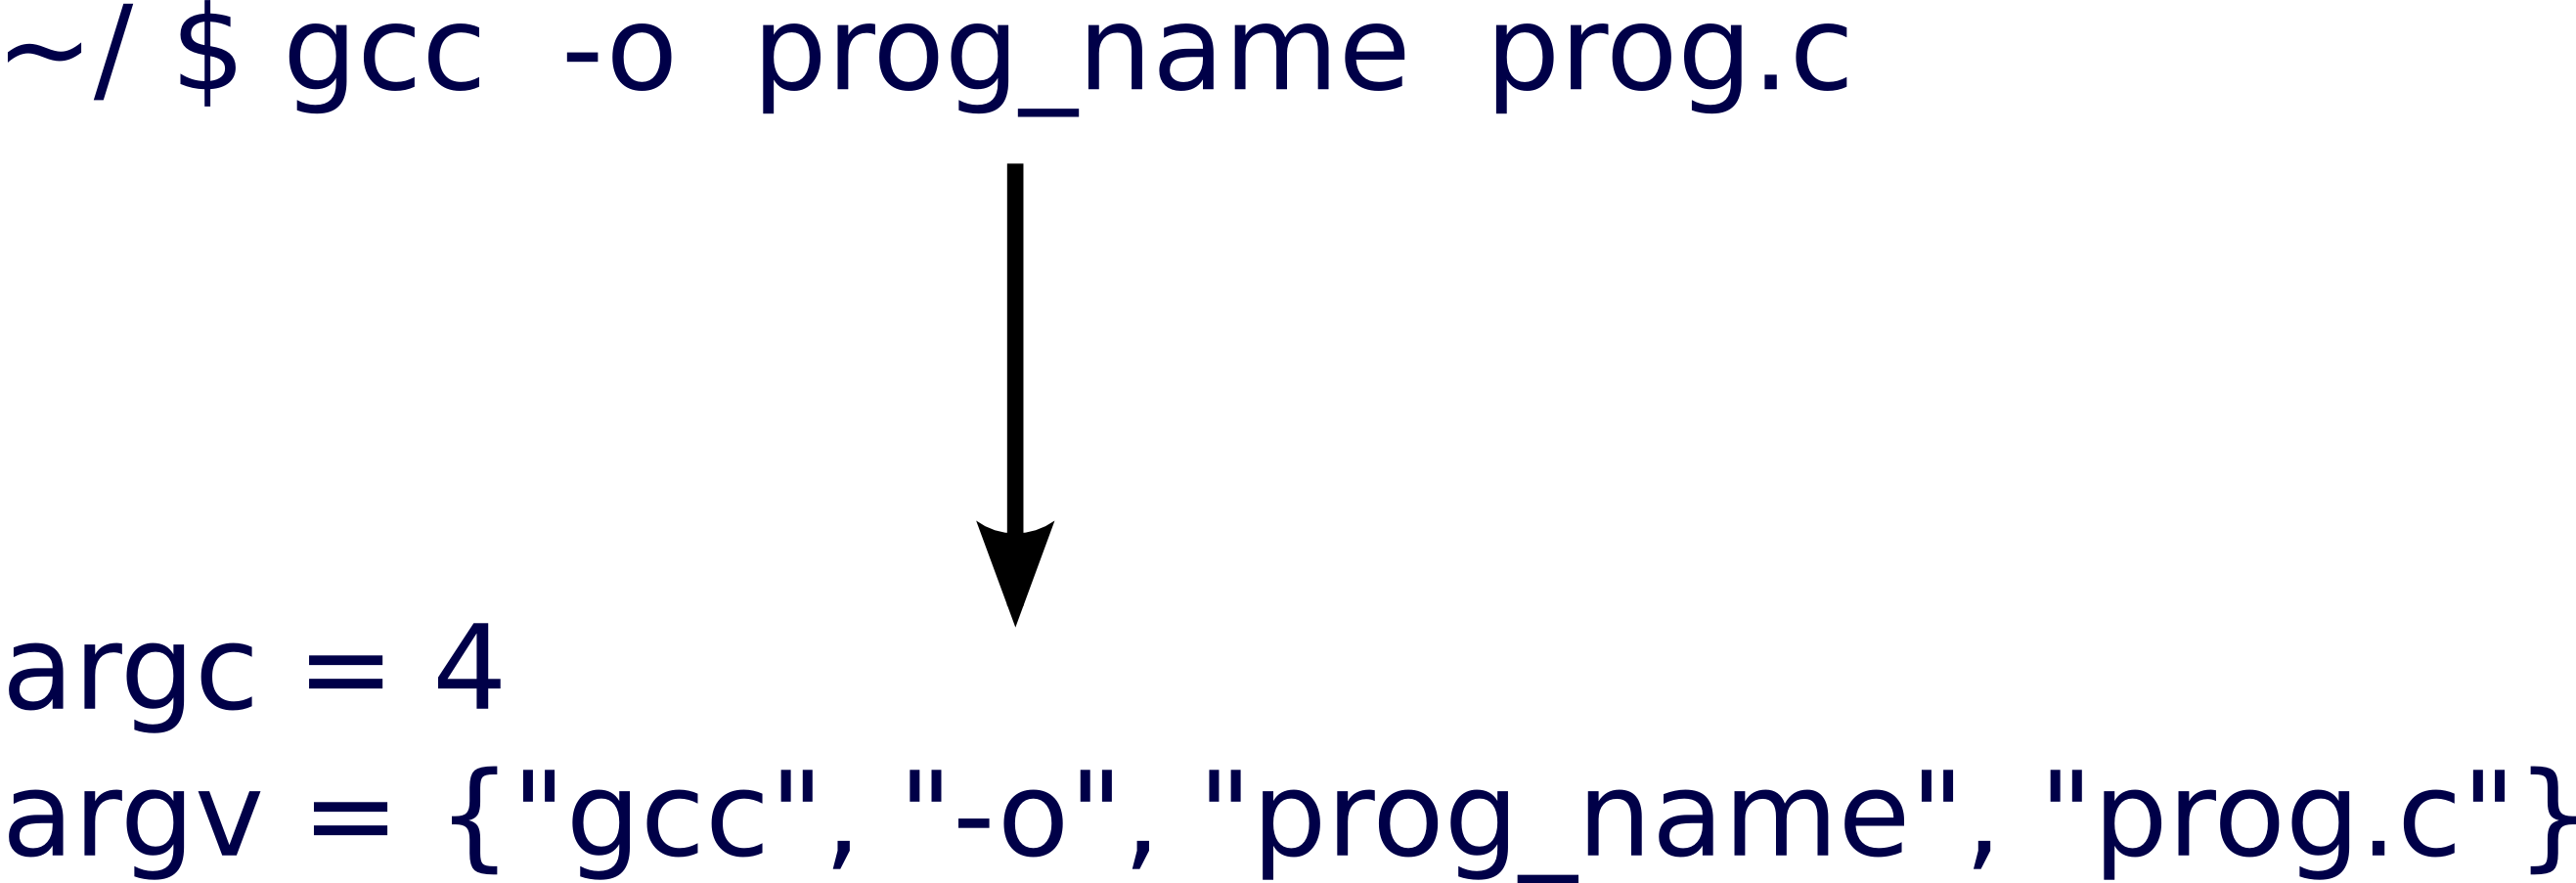
\includegraphics[width=1.0\linewidth]{images/function_argcargv.png}
\end{center}
\end{frame}
\fi

\iffalse
\section{Директивы препроцессора \#include и \#define}


\begin{frame}[fragile]
\frametitle{Препроцессор C} 
\begin{itemize}
\item Препроцессор C -- программа, подготавливающая код программы к компиляции
\end{itemize}
\begin{center}
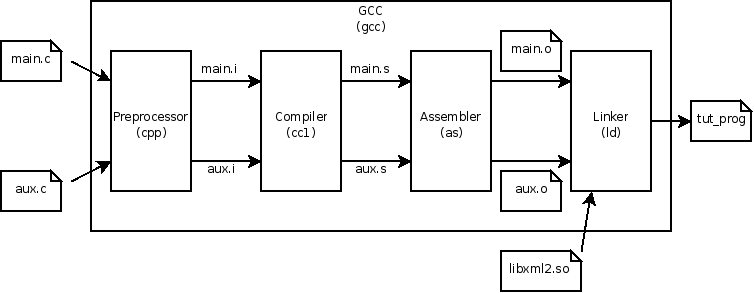
\includegraphics[width=0.95\linewidth]{images/compilation-stages.png}
\end{center}
\end{frame}


\begin{frame}[fragile]
\frametitle{Директива \#include} 
\begin{itemize}
\item Подставляет содержимое указанного файла на место этой директивы
\item \begin{lstlisting}[language=C,basicstyle=\ttfamily,keywordstyle=\color{blue}]
#include <stdio.h>
#include "my_file.txt"
\end{lstlisting}
\end{itemize}
\end{frame}

\begin{frame}[fragile]
\frametitle{Директива \#define -- макроподстановка} 
\begin{itemize}
\item Подставляет заданное выражение вместо заданного токена
\item \begin{lstlisting}[language=C,basicstyle=\ttfamily,keywordstyle=\color{blue}]
#define NUMBER_OF_MONTHS 12
#define LESS <
\end{lstlisting}
\item Часто используется для задания констант (особенно в старом коде)
\item С \#define нужно быть аккуратным
\end{itemize}
\end{frame}


\section{Квалификатор типа const}

\begin{frame}[fragile]
\frametitle{Квалификатор типа const} 
\frametitle{Современное задание констант}
\begin{lstlisting}[language=C,basicstyle=\ttfamily,keywordstyle=\color{blue}]
const int number_of_months = 12;
const float Pi = 3.14159265;
\end{lstlisting}
\end{frame}

\fi

\section{Рекурсия}


\begin{frame}[fragile]
\frametitle{Рекурсия} 
\begin{itemize}
\item Существует возможность вызвать функцию внутри самой функции
\item Tакой вызов функции называется рекурсивным
\end{itemize}
\end{frame}

\begin{frame}[fragile]
\frametitle{Рекурсия} 
\frametitle{Пример рекурсии: вычисление факториала} 
\begin{center}
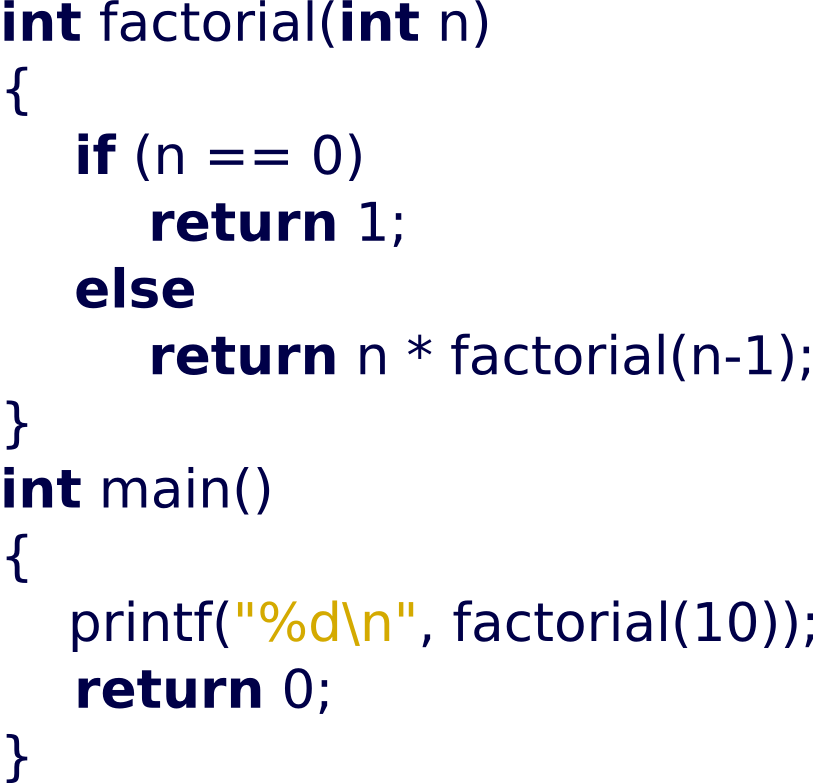
\includegraphics[width=0.65\linewidth]{images/function_recursive.png}
\end{center}
\end{frame}







\end{document}
